\documentclass[12pt]{article}

\usepackage{graphicx}
\usepackage{epstopdf}


\usepackage[spanish]{babel} % silabea palabras castellanas <- Puedo poner comentarios para explicar de que va este comando en la misma línea
\selectlanguage{spanish} 

%Encoding
\usepackage[utf8]{inputenc} % Acepta caracteres en castellano
\usepackage[T1]{fontenc} % Encoding de salida al pdf

%Triunfó el mal
\usepackage[normalem]{ulem}
\useunder{\uline}{\ul}{}
\providecommand{\e}[1]{\ensuremath{\times 10^{#1}}}
\usepackage{quotmark} %Uso consistente con la RAE de comillas
\usepackage{listings} % Comandos de la terminal

\usepackage{textcomp}
\usepackage{gensymb}


%Hipertexto
\usepackage[colorlinks=true,urlcolor=blue,linkcolor=blue]{hyperref} % navega por el doc: hipertexto y links

%Aquello de las urls
\usepackage{url} 

%simbolos matemáticos
\usepackage{amsmath}
\usepackage{amsfonts}
\usepackage{amssymb}
\usepackage{physics} %Best pack

% permite insertar gráficos, imágenes y figuras, en pdf o en eps
\usepackage{graphicx}
\usepackage{epstopdf}
\usepackage{multirow}
\usepackage{float}
\usepackage[export]{adjustbox}
% geometría del documento, encabezados y pies de páginas, márgenes
\usepackage{geometry}
\usepackage{comment}

%\usepackage[english]{babel}
%\usepackage[latin5]{inputenc}
% \usepackage{hyperref}
%\newdate{date}{10}{05}{2013}
%\date{\displaydate{date}}
\begin{document}




\title{Cúmulos Abiertos \\ Taller 3 Fotometría de Apertura IRAF}

\author{
\textbf{Javier Alejandro Acevedo Barroso\thanks{e-mail: \texttt{ja.acevedo12@uniandes.edu.co}}}\\
\textit{Universidad de los Andes, Bogotá, Colombia}\\
 }% Hasta aquí llega el bloque "author" (son dos autores por informe, orden alfabético)

\date{\today}
%\date{Versión $\alpha \beta$ fecha del documento}
\maketitle %Genera el título del documento


\normalsize
\newpage


\section{Fotometría de apertura}
El objetivo de este ejercicio es realizar la fotometría de apertura para las imágenes del tutorial de IRAF correspondientes al objeto M92.
Esto corresponde a calcular la magnitud instrumental para los objetos del campo estelar. Por ser la primera vez que se realiza tal análisis, se realizará paso a paso y para un número límitado de estrellas.
En futuros ejercicios se realizará el análisis para todo el campo, usando algoritmos implementados en IRAF para localizar los objetos.

Las imágenes se tomaron con instrumentos CCD y por lo tanto se realizaron las respectivas correcciones de FLAT, OVERSCAN, OFFSET y BIAS. El ejercicio asume que las imágenes ya están corregidas.


El primer paso va a ser añadir al header de las imágenes la masa de aire. El cálculo de la masa de aire requiere de cierta información como la posición del observatorio o la coordenada exacta en el cielo del objeto. Afortunadamente, IRAF incluye la tarea SETAIRMASS, la cual lee toda la información necesaria del header de la imagen y calcula la masa de aire. Usando la tarea SETAIRMASS y señalando que estamos en el observatorio \tqt{kpno} (Kitt Peak National Observatory), se fija en el header de cada imagen la masa de aire. Se observa que la masa de aire para las imágenes de calibración es de aproximadamente 2, esa masa de aire es irrelevante pues las imágenes de calibración no son tomas del cielo. Las masas de aire para las imágenes reales en el filtro V es 1.07 y en el filtro B 1.09.

Una vez fijada la masas de aire, se realizó la fotometría de apertura.
Para ello se utilizó el paquete DIGIPOT y APPHOT.
La fotometría se realizará sobre los objetos que creemos ser estrellas. Para seleccionar estrellas, se evaluaron las curvas de intensidad radiales de cada objeto candidato, y solo se tomó las estrellas con curvas coherentes con el perfil de una estrella.
Esto se hizo con la tarea IMEXAMINE.
Adicionalmente, se observó que las estrellas tienen un FWHM de 2.65 a 3.2 y que es constante entre las diferentes imágenes.
Por lo anterior, se usaron los siguientes parámetros para la fotometría:

\begin{table}[htb]
	\begin{tabular}{|c|c|c| }
	\hline
	Radio de apertura & Radio interior del anillo de cielo & Grosor del anillo de cielo  \\ \hline
	
		10 pixeles & 15 pixeles & 10 pixeles \\
	\hline
	\end{tabular}
\end{table}

Tras ejecutar la tarea QPHOT sobre la imagen m92010, se obtiene una tabla de objetos con sus coordenadas, su magnitud, y el resultado de la ejecución (\tqt{ok} o \tqt{err}). Usando la tarea txdump se extrae las coordenadas de las estrellas seleccionadas (se seleccionó a las estrellas en el modo interactivo de QPHOT). Una vez se tiene las coordenadas de las estrellas, se vuelve a correr QPHOT sobre las otras imágenes. Se seleccionaron 30 estrellas (ver figura \ref{im4}) para realizar la fotometría.



\begin{figure}[H]
\centering
   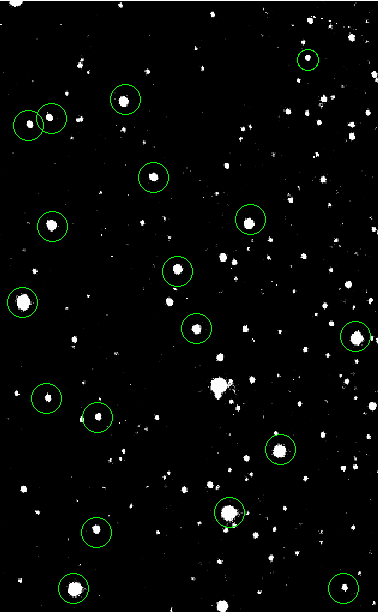
\includegraphics[scale=0.4]{imagenes.png}
  \caption{Estrellas seleccionadas para la fotometría de apertura en la imagen m92010.}
  \label{im4}
\end{figure}

Adicionalmente, para cada imagen se graficó magnitud contra la incertidumbre de la magnitud. En un análisis correcto se espera un comportamiento cuadrático en la gráfica $m$ vs $\Delta m $. Se observó el comportamiento cuadrático en todas las gráficas (ver figura \ref{im5}).


Por último, para verificar que el comportamiento cuadrático se debe a un análisis correcto, se calculó la magnitud y el error en la magnitud para coordenadas aleatorias del cielo, procurando no tomar estrellas. Se observó un comportamiento muy levemente cuadrático (probablemetne un remanente de las estrellas que sí quedaron a dentro de los circulos) y una gran cantidad de puntos indeterminados, debido a que el algoritmo no logra hayar una magnitud en esas coordenadas.

\begin{figure}[H]
   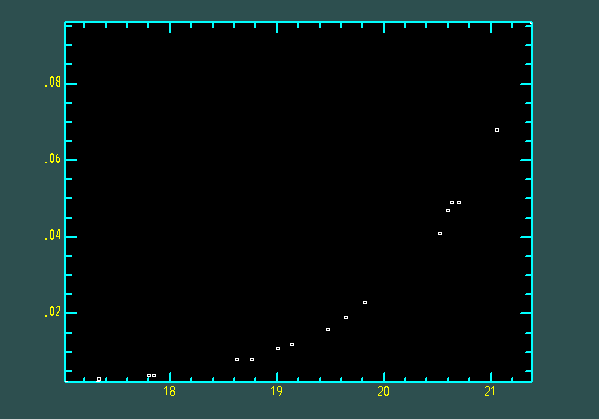
\includegraphics[scale=0.4]{mvsdm0.png}
   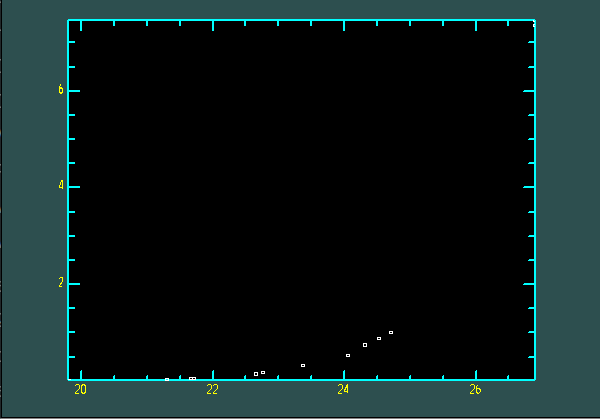
\includegraphics[scale=0.4]{mvsdm1.png}

  \caption{ A la izquierda magnitud contra incertidumbre en la magnitud para las estrellas en la imagen m92010. Se observa un comportamiento cuadrático. Se anexa únicamente el caso de m92010 porque las otras gráficas son muy similares. A la derecha la misma gráfica pero para puntos que no correspondieran a estrellas, la disminución de puntos se debe a que el algoritmo no converge en muchas ocasiones debido al ruido de fondo. Note que tanto la magnitud como la incertidumbre son considerablemente mayores.}
  \label{im5}
\end{figure}






%\bibliography{bibTes}{}
%\bibliographystyle{unsrt}



\end{document}




\begin{figure}[H]
  \centering
   \includegraphics[scale=•]{•}= 0.65]{im03.png}
  \caption{Cargando las imágenes a diferentes frames de DS9 desde la sesión de IRAF. }
  \label{im03}
\end{figure}





\section{Cronograma}

\begin{table}[htb]
	\begin{tabular}{|c|cccccccccccccccc| }
	\hline
	Tareas $\backslash$ Semanas & 1 & 2 & 3 & 4 & 5 & 6 & 7 & 8 & 9 & 10 & 11 & 12 & 13 & 14 & 15 & 16  \\
	\hline
	1 & X & X & X  &   &   &   &   &  &  &   &   &   &   &   &   &   \\
	2 &   &  & X & X & X &  &  &   &   &  &  &  &   &  &  &   \\
	3 &   &   &   &  & X  & X  & X  & X &   &   &   &  &   &   &  &   \\
	4 &  &  &  &  &  &  &  & X & X & X & X &   &   &   &   &   \\
    5 &  &  &  &  &  &  & X & X &  &  &  &   &   &   &   &   \\
	6 &   &   &   &   &  &   &  X & X  &  &   &  X & X &  X & X  & X &   \\
	\hline
	\end{tabular}
\end{table}
\vspace{1mm}
 %CCDRED se encarga de la corrección en sí, sus parámetros son: el tipo de dato de los pixeles (real, short, etc), el nombre del backup (en caso de querer un backup), el archivo de traducción del instrumento (que para una CCD estandar ya viene incluido en IRAF